% -*- coding: utf-8 -*-
% !TEX root = ../main.tex

% TODO Développer dans plusieurs sous-sections ce que vous avez réalisé pendant votre stage

\tcbFileInput{shell}{\faTerminal}{lst/hw.sh}{Exemple de script shell}{lst:hw}

% Alternative | Fonctionne avec la version 2025 de TeX Live
% \fileInput[%
%     language=shell,
%     logo=\faTerminal,
%     caption={Exemple de script shell},
%     label=lst:hw
% ]{lst/hw.sh}

\tcbFileInput{python}{\faPython}{lst/dummy.py}{Exemple de script Python}{lst:dummy}

\begin{figure}[!h]
\begin{center}
\tikzsetnextfilename{dummy}
\resizebox{\textwidth}{!}{%
% -*- coding: utf-8 -*-
% !TEX root = ../main.tex

\documentclass[tikz]{standalone}

%%%%%%%%%%%%%%%%%%%%%%%%%%%%%%%%%%%%%%%%
%%%%%%% DÉCLARATION DU PRÉAMBULE %%%%%%%
%%%%%%%%%%%%%%%%%%%%%%%%%%%%%%%%%%%%%%%%

\makeatletter
\def\input@path{{../}}
\makeatother

\usepackage{preamble}

%%%%%%%%%%%%%%%%%%%%%%%%%%%%%%%%%%%%%%%
%%%%%%%%%% DÉBUT DU DOCUMENT %%%%%%%%%%
%%%%%%%%%%%%%%%%%%%%%%%%%%%%%%%%%%%%%%%

\begin{document}

%%%%%%%%%%%%%%%%%%%%%%%%%%%%%%%%%%%%%%%
%%%%%%% DÉBUT DE L'ILLUSTRATION %%%%%%%
%%%%%%%%%%%%%%%%%%%%%%%%%%%%%%%%%%%%%%%

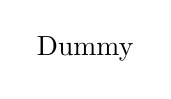
\begin{tikzpicture}
\node(dummy) {Dummy};
\end{tikzpicture}

%%%%%%%%%%%%%%%%%%%%%%%%%%%%%%%%%%%%%%%
%%%%%%%% FIN DE L'ILLUSTRATION %%%%%%%%
%%%%%%%%%%%%%%%%%%%%%%%%%%%%%%%%%%%%%%%

\end{document}

}%
\caption{Exemple de dessin TikZ}
\label{fig:dummy}
\end{center}
\end{figure}

On peut insérer du texte avec une image \inlinegraphics{example-image-a} et faire à la \autoref{sec:introduction}.

Paralléliser un code Python, c'est une bonne idée. \cite{mpi4py}

Je fais référence au glossaire par l'adjectif suivant : \gls{egal}, \glsf{egal}, \glspl{egal}, \glsf{egal}s.

%%%%%%%%%
%%%%%%%%%
%%%%%%%%%
%%%%%%%%%

\subsection{Parlons \glsentrytext{cpu}}\label{ssec:dummy_cpu}

On parlera aussi éventuellement du \gls{cpu}, du débit \acrshort{io} ou de l'espace de stockage en \acrlong{go}.

Connaissez-vous la fonction \( \gls{psi} \) ?
